%%
% このファイルは筑波大学情報学群情報科学類の卒業研究論文のサンプルです。
% このファイルを書き換えて、このサンプルと同様の書式の論文をLaTeXを使って
% 作成できます。
%
% OSやLaTeXの設定によっては漢字コードや改行コードを変更する必要があります。
%%
\documentclass[a4paper,11pt]{jreport}

%%【PDF, PostScript, JPEG, PNG等の画像の貼り込み】
%% dvipdfmx を使う場合
\usepackage[dvipdfmx]{graphicx}
%% dvipdfmx を使ってPDFの「しおり」を付ける場合
%%\usepackage[dvipdfmx,bookmarks=true,bookmarksnumbered=true,bookmarkstype=toc]{hyperref} \usepackage{pxjahyper}
\usepackage{ulem}
\usepackage{times} % use Times font instead of default one
\usepackage{algorithm}
\usepackage{algpseudocode}
\usepackage{amsmath}

\setcounter{tocdepth}{3}
\setcounter{page}{-1}

\setlength{\oddsidemargin}{0.1in}
\setlength{\evensidemargin}{0.1in}
\setlength{\topmargin}{0in}
\setlength{\textwidth}{6in}
%\setlength{\textheight}{10.1in}
\setlength{\parskip}{0em}
\setlength{\topsep}{0em}

\newcommand{\figref}[1]{図\ref{#1}}
\newcommand{\tabref}[1]{表\ref{#1}}
\newcommand{\secref}[1]{\ref{#1}節}
\newcommand{\algorithmref}[1]{Algorithm \ref{#1}}
\newcommand{\equationref}[1]{式(\ref{#1})}

%% タイトル生成用パッケージ(重要)
\usepackage{coins}

%% タイトル
\title{進化的計算による \ 輻輳制御アルゴリズムの探索手法の提案}
%% 著者
\author{岡部 純弥}
%% 指導教員
\advisor{岡 瑞起, 阿部 洋丈}

%% 年度と主専攻名
\fiscalyear{2024}
\majorfield{ソフトウェアサイエンス主専攻}

\begin{document}
\maketitle
\thispagestyle{empty}
\newpage

\thispagestyle{empty}
\vspace*{20pt plus 1fil}
\parindent=1zw
\noindent
%%
%% 論文の要旨
%%
\begin{center}
{\Large \bf 要  旨}
\vspace{2cm}
\end{center}

優れた輻輳制御アルゴリズムを発見することは難しい。主な理由として、コンピュータネットワークの構造が時々刻々と変化することが挙げられる。つまり、特定のネットワーク構造化で最適なアルゴリズムを探索しても、時間経過につれ、良いパフォーマンスを発揮できなくなってしまう。

そこで、大規模言語モデルと進化アルゴリズムを用いることで任意のネットワーク環境下で最適化を行う探索手法を提案する。既存の探索手法では、探索空間の制約が厳しかったものの、大規模言語モデルを用いることで、この問題を解決できた。

TODO: 事実確認

実際にネットワークシミュレータを用いた実験を行い、ベンチマークを超える輻輳制御アルゴリズムを発見できた。

%%%%%
\par
\vspace{0pt plus 1fil}
\newpage

\pagenumbering{roman} % I, II, III, IV
\tableofcontents
\listoffigures
%\listoftables

\pagebreak \setcounter{page}{1}
\pagenumbering{arabic} % 1,2,3

\chapter{序論}

\section{研究背景}

TCP/IPネットワークでは、トランスポート層で輻輳制御が行われている。輻輳制御の難しさとして、限られた観測可能な値から、観測不可能な状態を推定しなければならないことが挙げられる。
つまり、限られた観測値から、輻輳が発生しているのかを判断したうえで、パケット送信量を制御しなければなければならない。

さらに、ネットワーク構造が変化し続けているため、支配的なアルゴリズムが存在することもなく、数年に一度はパラダイムシフトが起こっている。

現在の輻輳制御アルゴリズムの探索、発見は、ヒューリスティックに行われている側面があり、人的リソースを割き続けなければらない。つまり、ネットワーク構造の変化に柔軟に対応可能な探索手法の発見が求められている。

\newpage

\section{本論文の構成}

第2章の前半では、輻輳制御アルゴリズムの概要や、その発展について述べる。
第2章の後半では、近年の大規模言語モデルの発展や、その応用について概説する。特に、輻輳制御アルゴリズムの探索手法として、大規模言語モデルを用いることの可能性について述べる。
第3章では、これらの関連研究を踏まえたうえでの仮説、および提案手法について述べる。
第4章では、仮説を検証するために提案手法の実装、実験の詳細について述べる。
第5章では、実験結果を示し、その結果に対する考察を行う。
第6章では、本論文のまとめと今後の課題について述べる。

\newpage

\chapter{関連研究}
\section{輻輳制御アルゴリズム}

\subsection{輻輳制御アルゴリズムの概要}

% TODO: 表現の見直し
パケット交換型の通信網であるTCP/IPネットワークでは、トランスポート層で輻輳制御が行われている。
そもそも輻輳とは、ネットワーク上のあるノード
\footnote{多くの場合、これは中継ルータのいずれかである。}
で、パケットが過剰に蓄積されパケットロスが発生、あるいはパケットの遅延が発生する状態のことを指す。
一般的に、ルータ上ではパケットを蓄積するためのバッファが存在しており、これは FIFO: First In First Out 型のキューであるため、このバッファが溢れるとパケットのロスが発生する。
TCP/IPにおいて、トランスポート層では通信の信頼性を確保するために、パケットロスを検知するとパケットが再送される。
このため輻輳が発生すると、パケットロスが発生し通信のスループットが低下する。
\footnote{よりひどい状態になると、輻輳崩壊と呼ばれる状態になり、大規模な通信障害を引き起こすこともある。}
このような状態を回避するため
\footnote{Chiuら\cite{CHIU19891}は、単純な加算的増加、乗算的減少のアルゴリズムが、ネットワークの状態に関係なく効率的に輻輳回避に貢献することを検証した。}
に、輻輳制御という仕組みが存在する。

輻輳制御\cite{congestion-avoidance}は、観測可能な値からネットワークの状態を推定し、一度に送信するパケットの量を制御する。
多くの場合、輻輳制御によって輻輳の発生を抑えることができる
\footnote{実際にJacobson\cite{congestion-avoidance}で提案された、世界初の輻輳制御アルゴリズムは、TCP Tahoeと名付けられた。}
。万が一輻輳が発生した場合には、輻輳制御アルゴリズムは輻輳が発生していることを検知してパケット送信量を制御し、輻輳の影響を抑える。
興味深いことに、Kellyら\cite{kelly1998rate}は、全体最適化やゲーム理論の観点から、各々のノードが自身のパケット送信量を制御することでネットワーク全体としてのスループットを最大化できることを示した。
それゆえ現在の輻輳制御アルゴリズムは、OSのカーネルに実装されており、自分自身のパケット送信量を制御のみを行うことが多い。

単純な輻輳制御アルゴリズムの動作を\algorithmref{algorithm:congestion_control_algorithm}に示す。
\begin{algorithm}
  \caption{Basic Congestion Control Algorithm}
  \label{algorithm:congestion_control_algorithm}
  \begin{algorithmic}[1]
  \State $windowSize \gets 1$
  \State $threshold \gets veryLargeNumber$
  \While{true}
      \If{ACK is received}
        \If{$windowSize < threshold$}
            \State $windowSize \gets windowSize + 1$
        \Else
            \State $windowSize \gets windowSize \times 2$
        \EndIf
      \EndIf
      \If{Congestion is detected}
          \State $threshold \gets windowSize / 2$
          \State $windowSize \gets 1$
      \EndIf
  \EndWhile
  \end{algorithmic}
\end{algorithm}
\algorithmref{algorithm:congestion_control_algorithm}では、以下の2つの変数と、ACKの受信の契機によってパケットの送信量を調整する。

% TODO: windowSize ではなく、cwnd と書く
% TODO: threshold ではなく、ssthresh と書く

\begin{description}
  \item[windowSize] windowSizeは、一度に送信可能なパケットの数を表す。輻輳制御アルゴリズムは、このwindowSizeを制御することで、パケット送信量を制御する。
  \item[threshold] thresholdは、windowSizeを指数関数的に増加させる際の閾値を表す。thresholdを超えた場合には、windowSizeは加算によって増加させる。
\end{description}
\algorithmref{algorithm:congestion_control_algorithm}では、輻輳が発生していない場合にはwindowSizeを指数的あるいは線形に増加させることでパケット送信量を増加させる。
一方で輻輳が発生した場合には、windowSizeを減少させることで、パケット送信量を減少させる。
これが、輻輳制御アルゴリズムの基本的な動作である。

\subsection{代表的な輻輳制御アルゴリズム}

ここでは、代表的な輻輳制御アルゴリズムについて概説する。
輻輳制御アルゴリズムは、大きくLoss-basedとDelay-basedに分類される。
これは輻輳制御アルゴリズムがどのように輻輳を検知するかによって分類されており、Loss-basedはパケットロスを検知することで輻輳を検知する。
一方で、Delay-basedは、RTT: Round Trip Time
\footnote{パケットが送信元から受信元に送信され、さらにそのACKが送信元に返ってくるまでの合計時間のことを指す。}
を用いることで輻輳を検知する。
それぞれの代表的な輻輳制御アルゴリズムについて、\figref{figure:congestion_control_classification}に示す。
\begin{figure}[htbp]
  \centering
  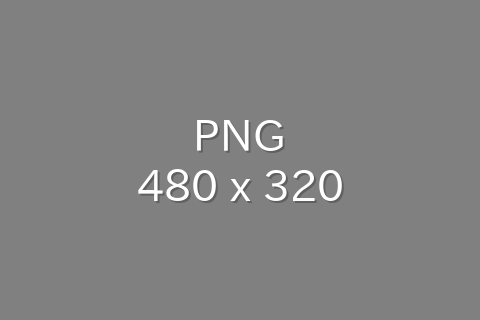
\includegraphics[width=0.6\linewidth]{fig/chap02/empty.png}
  \caption{[wip] 輻輳制御アルゴリズムの分類}
  \label{figure:congestion_control_classification}
\end{figure}
\figref{figure:congestion_control_classification} では、Loss-based 輻輳制御アルゴリズムをhoge色で、Delay-based 輻輳制御アルゴリズムをfuga色で示している。

\subsubsection*{Loss-based 輻輳制御アルゴリズム}

Loss-basedの代表的な輻輳制御アルゴリズムとしては、TCP Reno\cite{reno,tcp}が挙げられる。
これは、TCP Tahoe\cite{congestion-avoidance}を改良したもので、Fast RetransmitとFast Recoveryという機構を追加したものである。
これらはTCP Tahoeの課題であった、輻輳発生後のwindowSizeの回復速度を改善するために追加された。
% TCP Renoの動作の概要を\figref{figure:reno-timeline}に示す。
% \begin{figure}[htbp]
%   \centering
%   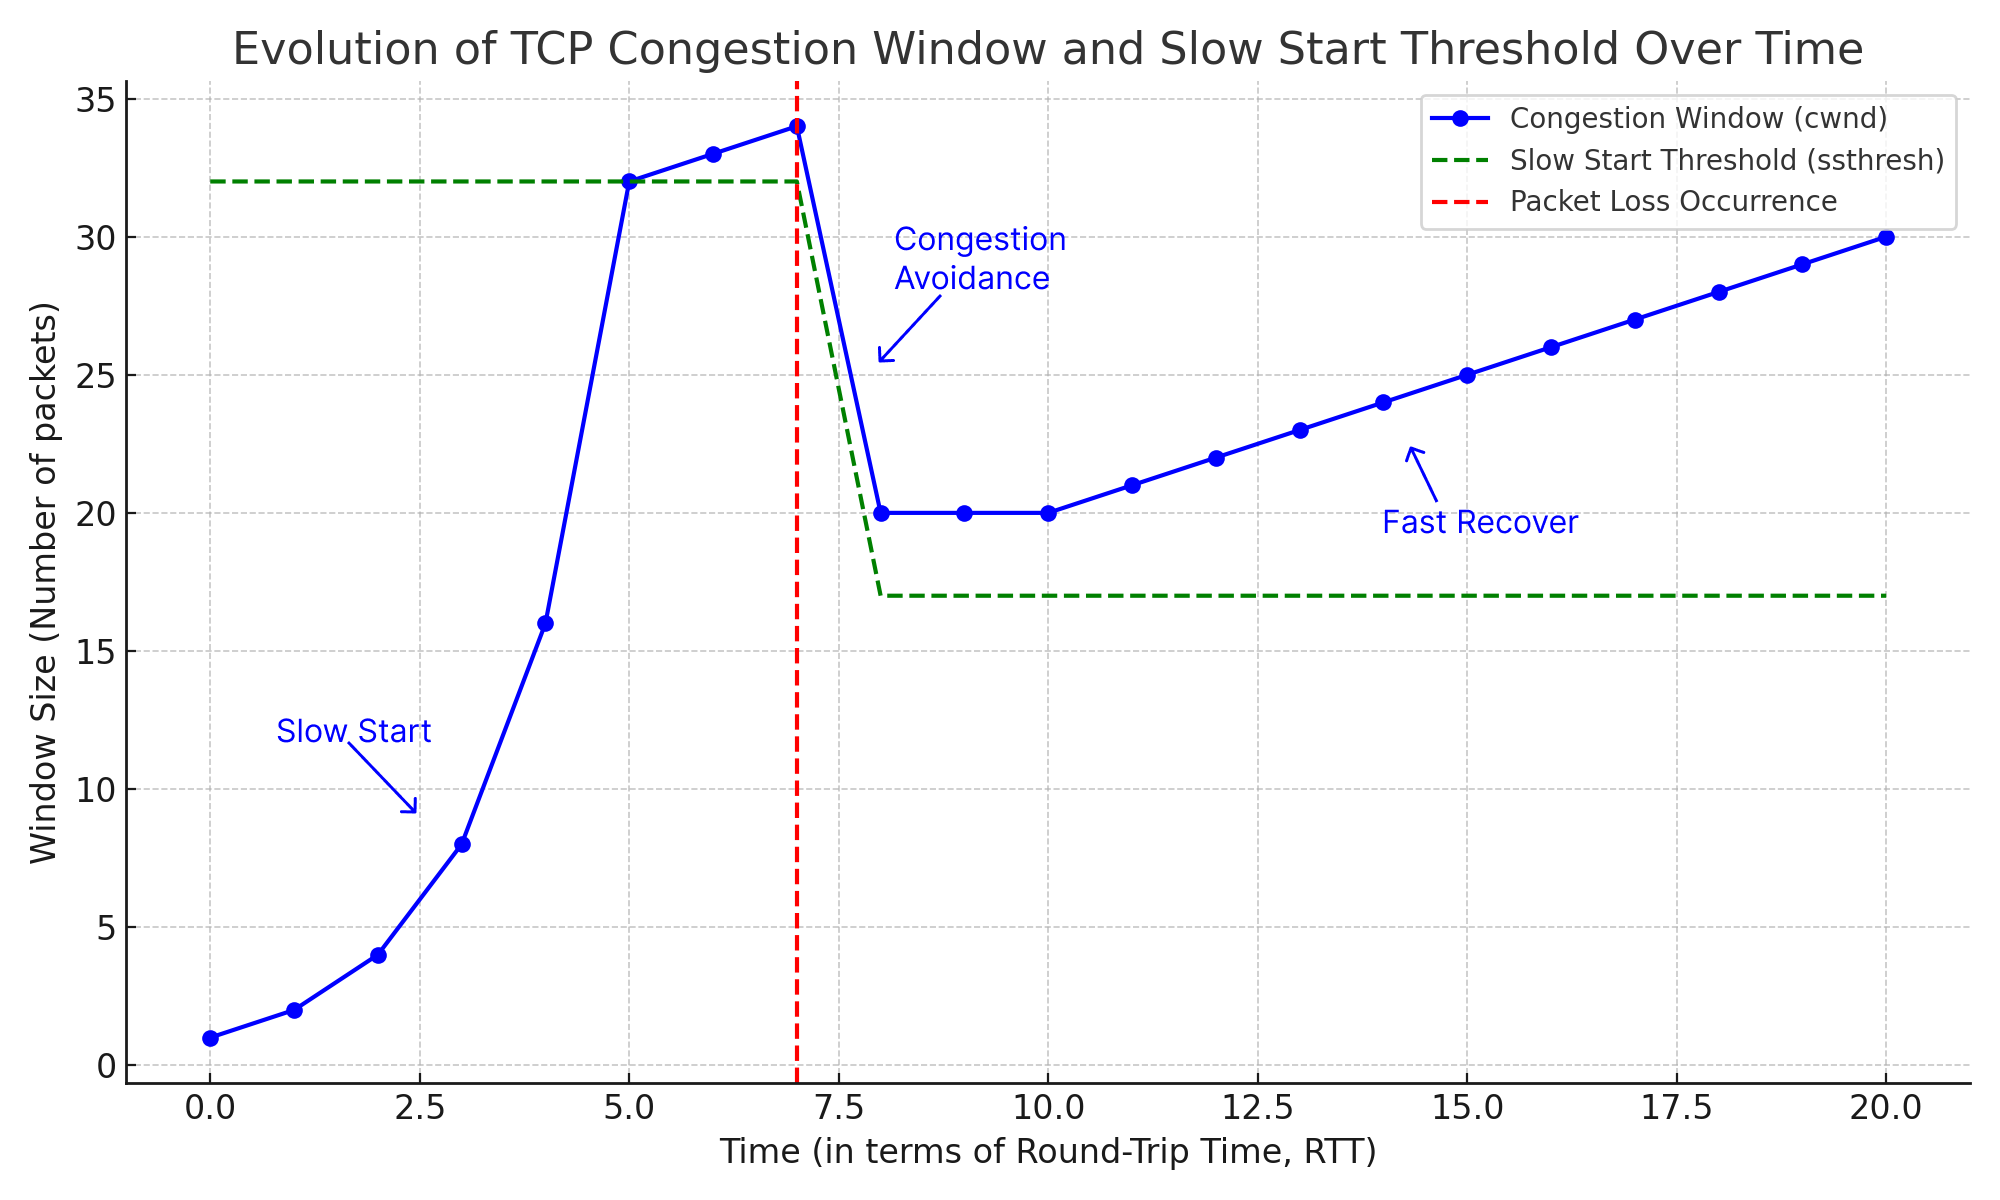
\includegraphics[width=0.6\linewidth]{fig/chap02/CongestionControlAlgorithm_Timeline.png}
%   \caption{TCP Renoの動作の概要}
%   \label{figure:reno-timeline}
% \end{figure}
% TODO: \figref{figure:reno-timeline}の説明

TCP Renoをさらに改良したTCP NewReno\cite{floyd2004newreno,henderson2012newreno}では、Fast Recoveryの実装やパケット損失時のwindowSizeの回復方法が改良されている。
特に複数のパケットの損失時のwindowSizeの回復方法が改良されている。
TCP RenoではFast Recover中に他のパケットが損失した場合、その損失は検出されず、ACKが受信されるまでwindowSizeが回復しない。
一方で、TCP NewRenoではFast Recover中でも他のパケットに対する処理が行われるため、損失が検出されるとすぐにwindowSizeが回復する。

\subsubsection*{Delay-based 輻輳制御アルゴリズム}

一方で、Delay-basedの代表的な輻輳制御アルゴリズムとしては、TCP Vegas\cite{tcp-vegas}やBBR\cite{bbr}が挙げられる。
Delay-basedの輻輳制御アルゴリズムは、パケットロスを検知するのではなくRTTによってネットワーク上の輻輳の程度を推定し、パケット送信量を制御する。

TCP Vegasは、RTTの変化量を用いて輻輳を検出する。
RTTの変化による輻輳の検知は、一般的にはパケットロスによる検知よりも早いため、windowSizeの調整をより早く行うことができる
\footnote{実際には、Delay-basedな輻輳制御アルゴリズムの輻輳の検知がLoss-basedよりも早いことで、パフォーマンス上の問題が発生することがある。
例えばTCP Renoと、TCP Vegasが共存するネットワークにおいて、TCP VegasがRTTの変化によって素早くwindowSizeを調整する一方で、TCP Renoはパケットロスが発生するまで、多くのパケットを送信し続ける。
それゆえ、帯域幅の多くをTCP Renoが占有することになり、TCP Vegasのパフォーマンスが低下することがある。
}
。それゆえ、帯域幅を効率的に利用することができる。
TCP Vegasのウインドウサイズの更新式を、\equationref{equation:tcp-vegas}に示す
\footnote{論文によっては、更新幅を1ではなく、$1/cwnd$としていることがある。
$1/cwnd$にすることで、$cwnd$が大きくなった際の更新幅を小さくし、輻輳の発生を抑制する効果がある。}。
ただし、$\alpha$と$\beta$は閾値を表す定数で、$\alpha \leq \beta$である。
\begin{equation}
  \label{equation:tcp-vegas}
  cwnd_{now} =
  \begin{cases}
    cwnd + 1 & \text{if } diff < \alpha \\
    cwnd - 1 & \text{if } diff > \beta \\
    cwnd & \text{otherwise}
  \end{cases}
\end{equation}
ここで、$diff$はRTTを元に推定される転送データの量であり、\equationref{equation:diff}に示すように計算される。
\equationref{equation:diff}の$RTT'$は、RTTの最小値を表す。
\begin{equation}
  \label{equation:diff}
  diff = \left( \frac{cwnd}{RTT'} - \frac{cwnd}{RTT}\right) RTT'
\end{equation}

BBR: Bottleneck Bandwidth and Round-trip propagation time は、Googleによって開発された輻輳制御アルゴリズムであり、従来の輻輳制御アルゴリズムとは異なるアプローチを採用している。
BBRでは、ボトルネックリンクの帯域幅
\footnote{経路上で最も低い値をとる帯域幅のことを指す。}
と往復時間遅延(RTproop: Round-trip propagation time)を推定し、これらの値を用いてパケット送信量を制御する。
BBRは、他のBBRを用いるノードとの通信において、公平性を保ちながら高いスループットと低遅延を実現できるためLinuxカーネル内でも実装されており、近年その採用が進んでいる。
一方で、他の輻輳制御アルゴリズムと共存した際に、BBRが帯域幅を占有する傾向にあることが指摘されている。

\subsubsection*{輻輳制御アルゴリズムの性能評価}

輻輳制御アルゴリズムの性能評価に関して、ネットワーク環境や評価指標など様々な観点から研究が行われている。
ネットワーク構造の変化や接続形態の変化、支配的な輻輳制御アルゴリズムの変化など多くの要因が輻輳制御アルゴリズムの性能に影響を与えるため、その評価は難しい。
輻輳制御アルゴリズムの性能評価について、Fallら\cite{fall1996simulation}は、SACK: Selective Acknowledgement ~\cite{rfc2018}を用いたシミュレーションに基づく輻輳制御アルゴリズムの性能を評価した。Moら\cite{752178}は、TCP Vegasの性能評価をネットワークの公平性の観点から行い、いくつかの改良点を提案した。

より詳細な輻輳制御アルゴリズムの概説や近年の研究の動向については、Lowら\cite{980245}やGhaffari\cite{GHAFFARI2015101}などを参照されたい。

\section{大規模言語モデルと進化アルゴリズム}

\subsection{大規模言語モデル}

近年、大規模言語モデルの発展が著しい。
自然言語処理の分野における機械翻訳のタスクは、もともとはRNN\cite{graves2014generating}やLSTM\cite{6795963}などの時系列モデルを用いて行われていた。
しかし、これらの手法では長期的な依存関係を捉えることが難しく、特に長い文章を高精度に翻訳できなかった。
2017年、Vaswaniら\cite{attention}の提案した、Transformerと呼ばれるモデルがこの問題を解決した。
Transformerは、Attentionと呼ばれる機構を用いて、長期的な依存関係を捉えることができる。
さらに、Transformerは、既存モデルと比べて並列化が容易であるため、学習にかかる時間を短縮できる。

さらに、Devlinら\cite{devlin2019bert}は、Transformerをベースとした、BERTと呼ばれる手法を提案した。
Brownら\cite{gpt3}は、GPT3と呼ばれるモデルを提案した。
これらのモデルは大規模なコーパスを用いて学習されており、様々なタスクで既存のモデルを凌駕する性能を発揮した。
現在では特にgpt3の系統のモデルを中心に、これらは大規模言語モデル(LLM: Large Language Model)と呼ばれており、その性能は言うまでもないものなっている。
また大規模言語モデルは、自然言語処理分野にとどまらず画像処理分野や音声処理分野などにも応用されている。

\subsection{進化アルゴリズム}

遺伝的アルゴリズム(GA: Genetic Algorithm)\cite{genetic-algorithm, vose1999simple}は、生物の進化を模倣したアルゴリズムであり、進化アルゴリズムの一種である。
特に最適化問題において、広く用いられている
\footnote{遺伝的アルゴリズムは古典的な手法であるため、多くの場合、より優れた探索手法が存在する。しかし、遺伝的アルゴリズムはその実装の容易さや、過去の研究の蓄積などから、最適化問題において広く用いられている。}
。
GAは、個体群の中から適応度の高い個体を選択し、交叉や突然変異といった進化演算子を用いて新たな個体を生成する。
一般的な進化演算子は以下のようなものがある。
\begin{description}
  \item[選択]
  個体群の中から、次世代に残す個体を選択する。多くの場合、適応度が高い個体ほど選択されやすい。
  \item[交叉] 2つの個体を選択し、それらの遺伝子を交換する。一様交叉や2点交叉などの方法がある。
  \item[突然変異] 遺伝子の一部をランダムに変更する。
\end{description}
遺伝的アルゴリズムは、これらの進化演算子を用いて個体群を進化させ、最適解を探索する。
より詳しい遺伝的アルゴリズムの総説や、近年の応用については、Katochら\cite{katoch2021review}を参照されたい。

\subsection{進化アルゴリズムへの大規模言語モデルの応用}

近年、大規模言語モデルを用いて、進化アルゴリズムの進化演算子を実現する研究が行われている。Meyersonら\cite{meyerson2023language}は、進化演算における交叉を大規模言語モデルを用いて実現できるのかを検証し、いくつかの分野の問題
\footnote{数式生成のタスクや、画像処理、ソースコードの生成など}
において、これがうまく機能することを示した。
Lehmanら\cite{lehman2022evolution}は、大規模言語モデルを用いた変異によって、進化アルゴリズムがうまく機能するかを検証し、これを示した。

つまり単純なタスクであれば、進化アルゴリズムにおける交叉や変異を、大規模言語モデルを用いて実現できることが示されている。
特に変異においては、大規模言語モデルを用いることで、従来の手法より探索空間が広がりやすく、より多様な解を探索できることが示されている。

\subsection{進化アルゴリズムの輻輳制御アルゴリズムへの応用}

進化アルゴリズムや強化学習を用いて、輻輳制御アルゴリズムを探索する研究がいくつか行われている。
Endoら\cite{endo-2022-toward}は、遺伝的プログラミング\cite{holland1992adaptation, gp, gp-foundation}
\footnote{厳密には、GE (Grammatical Evolution) \cite{grammatical-evolution}と呼ばれる、遺伝的プログラミングの一種を用いている。GE では、プログラムの文法をBNF (Backus-Naur Form) で表現し、定義された文法に従ってプログラムを生成する。}
と品質多様性アルゴリズム\cite{quality-diversity}、共進化アルゴリズム\cite{poet, poet-gecco}を用いた輻輳制御アルゴリズムの探索を行った。

Endoらの研究では、実行可能な輻輳制御アルゴリズムを探索することに成功していたものの、遺伝的プログラミングを用いていたため、探索空間が限定されていたという問題があった。
Endoらの研究に限らず、遺伝的プログラミングや強化学習を用いた輻輳制御アルゴリズムの探索では、探索空間が限定されていることが多い。
これは文法をあらかじめ定義していることや、交叉や変異がAST: Abstract Syntax Treeに対する操作に限定されていることが原因である。
この問題に対する解決策を次章で検討する。

\newpage

\chapter{仮説}

関連研究をもとに、以下の仮説を立てた。
\begin{enumerate}
  \item 大規模言語モデルを用いた輻輳制御アルゴリズムの探索手法は、既存の探索手法と比べて、探索空間が広がるのではないか
  \item 進化アルゴリズム、特に遺伝的アルゴリズムを用いることで、既存の探索手法よりも多様かつ優れた輻輳制御アルゴリズムを発見できるのではないか
  \item 1, 2で提案した探索手法であれば、任意のネットワーク環境下
  \footnote{実験を行うネットワークシミュレータ上で環境を再現できる場合に限り}
  で最適な輻輳制御アルゴリズムを発見できるのではないか
\end{enumerate}
つまり、``大規模言語モデルを用いて交叉や変異を行う遺伝的アルゴリズムを用いて、輻輳制御アルゴリズムを探索する''という探索手法を提案する。
提案手法の概要を\figref{figure:proposed_flow}に示す。
\begin{figure}[htbp]
  \centering
  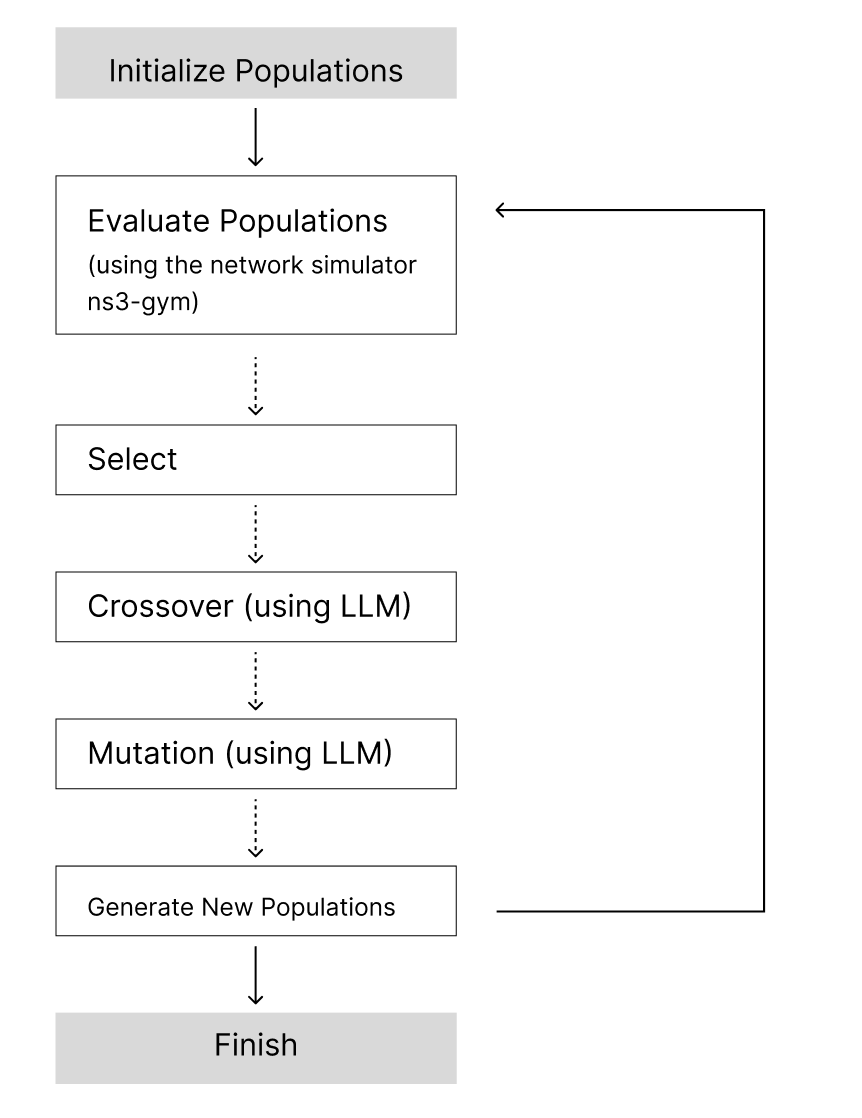
\includegraphics[width=0.4\linewidth]{fig/chap03/proposed_flow.png}
  \caption{提案手法の概要}
  \label{figure:proposed_flow}
\end{figure}
この提案手法は、既存の探索手法よりも、探索空間が広がり多様かつ優れた輻輳制御アルゴリズムを発見できるのではないか。

ソースコードで表現されるアルゴリズムを進化計算によって探索する場合、遺伝的プログラミング(GP: Genetic Programming)が用いられることが多い。
しかしGPでは、ソースコードを木構造によって表現しており、交叉や変異は木構造に対する操作となるため、探索空間が厳しく制限されてしまう。
変異によって木構造の一部が別の木構造に置き換えられることがあるが、それでも探索空間は制限されてしまう。

大規模言語モデルを用いた交叉や変異は、この探索空間上の制約が緩和されるのではないか。
さらに、特に変異において、有意な変化が起こる確率が高くなるのではないか。
この仮説を検証するために、大規模言語モデルを用いた遺伝的アルゴリズムを実装し、ネットワークシミュレータns3\cite{ns3-2012, ns3-2010}を拡張したns3-gym\cite{ns3gym}を用いて実験を行った。

\newpage

\chapter{実験}

この章では、実験の環境や実験方法、実装の詳細やその評価方法について述べる。

\section{実験環境}

\subsection{ネットワークシミュレータ}

本研究では、ネットワークシミュレータとして、ns3-gym\cite{ns3gym}を用いた。
ns3-gymは、ns3\cite{ns3-2012, ns3-2010}を拡張したもので、OpenAI Gym\cite{gym}
\footnote{現在はOpenAI Gymの開発は終了しており、Gymnasiumへの移行が進められている。}
のインターフェースを提供する
\footnote{つまり、ns3-gymでは輻輳制御アルゴリズムはPythonで表現され、これをns3のシミュレーションに組み込むことができる。
後述するOpenAIのgptモデルのAPI用ライブラリはPythonとnode.jsでのみ提供されているため、Pythonで実装されたns3-gymを用いた。
}。

% TODO: なんか追記するか別途考える

\subsection{大規模言語モデル}

本研究では、大規模言語モデルとしてOpenAIが提供するGPT-4を用いた。
GPT-4\cite{gpt4}は、2023年5月にリリースされたモデルで、多くのベンチマークでGPT-3よりも高い性能を発揮している。
この実験を行っている2023年11月現在、OpenAIが提供するモデルの中では最も性能が高いため、本研究ではGPT-4を用いる。
GPT-4はシンプルなJSON over HTTP(s) APIを提供している。
さらに、Pythonとnode.js用のAPI用ライブラリを公式に提供している。
したがって、本研究ではPythonを用いてPythonスクリプトからGPT-4のAPIを呼び出すことで、大規模言語モデルを利用する。

\subsection{実行環境}

本研究の実験は、以下のマシン上で行った。
また、Pythonのバージョンは3.11.6を用いた。

\begin{description}
  \item[CPU] Intel(R) Core(TM) i7-8700K CPU @ 3.70GHz
  \item[GPU] NVIDIA GeForce RTX 2080
  \item[メモリ] 64GB
  \item[OS] Ubuntu 22.04 LTS
\end{description}

\section{実験条件}
% ref. https://github.com/Okabe-Junya/ns3-gym/blob/master/scratch/rl-tcp/sim.cc
tcpEnvTimeStep = 0.01;
bottleneck\_bandwidth = "2Mbps";
bottleneck\_delay = "0.01ms";
access\_bandwidth = "10Mbps";
access\_delay = "20ms";
mtu\_bytes = 400;
duration = 10.0;
flow\_monitor = false;
sack = true;


\section{実験方法}

\section{評価方法}

\newpage

\chapter*{謝辞}
\addcontentsline{toc}{chapter}{\numberline{}謝辞}

本研究を行うにあたって、研究テーマの決定、研究内容の議論、外部発表の機会の提供など、様々な形でご指導を頂いた岡瑞起准教授、阿部洋丈准教授の両先生に深く感謝を申し上げます。
また、同研究プロジェクトの中で議論した、岡研究室の矢内千陽さん、OSSS研究室の佐藤創太さんの両氏にも感謝を申し上げます。
ネットワークシミュレータの取り扱いや実験環境に関して、OSSS研OBの森越さんには多大なるご協力を頂きました。
実験用のマシンのセットアップ等に関して、OSSS研の山本さん、広瀬さんには大変お世話になりました。
この場を借りて、深く御礼申し上げます。

そして、日々の研究活動やミーティングにおいて、様々な形でご協力を頂いた岡研究室の皆様、OSSS研究室の皆様にもあらためて感謝申し上げます。

\newpage

\addcontentsline{toc}{chapter}{\numberline{}参考文献}
\renewcommand{\bibname}{参考文献}

\bibliographystyle{junsrt}
\bibliography{ref.bib}

\end{document}
